\usetikzlibrary{arrows.meta, positioning}
\begin{figure*}
  \centering
  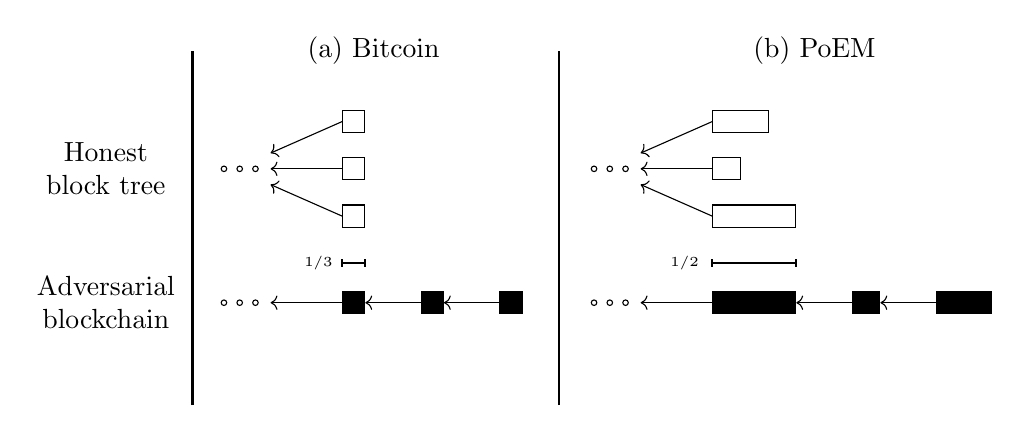
\begin{tikzpicture}

  % Define styles
  \tikzstyle{dot} = [circle, draw, fill=white, minimum size=2pt, inner sep=0pt]
  \tikzstyle{block} = [rectangle, draw, minimum size=8pt]
  \tikzstyle{adv_block} = [rectangle, draw, fill=black, minimum size=8pt]
  \tikzstyle{dashed_line} = [draw, dashed, thick]

  % Labels
  \node at (1.4, 5.5) {(a) Bitcoin};
  \node[align=center] at (-2, 4) {Honest \\ block tree};
  \node[align=center] at (-2, 2.3) {Adversarial \\ blockchain};

  \draw[thick] (-0.9, 1) -- (-0.9, 5.5);

  % Bitcoin Honest
  \node[dot, fill] (dot1) at (-0.5, 4) {};
  \node[dot] (dot2) at (-0.3, 4) {};
  \node[dot] (dot3) at (-0.1, 4) {};

  \node[block, anchor=west] (h2) at (1, 4) {};
  \node[block, anchor=west] (h1) at (1, 4.6) {};
  \node[block, anchor=west] (h3) at (1, 3.4) {};

  % Honest tree connections
  \draw[<-] (dot3.east) ++(0.15,0.2) -- (h1.west);
  \draw[<-] (dot3.east) ++(0.15,0) -- (h2.west);
  \draw[<-] (dot3.east) ++(0.15,-0.2) -- (h3.west);

  % Bitcoin Adversary
  \node[dot, fill] (dot1) at (-0.5, 2.3) {};
  \node[dot] (dot2) at (-0.3, 2.3) {};
  \node[dot] (dot3) at (-0.1, 2.3) {};

  \node[adv_block, anchor=west] (a1) at (1, 2.3) {};
  \node[adv_block, anchor=west] (a2) [right=20pt of a1] {};
  \node[adv_block, anchor=west] (a3) [right=20pt of a2] {};

  % Adversarial chain connections
  \draw[<-] (dot3.east) ++(0.15,0) -- (a1.west);
  \draw[<-] (a1) -- (a2);
  \draw[<-] (a2) -- (a3);

  % Bracket for Bitcoin (1/3)
  \draw[thick] (a1.west) ++(0.0,0.5) -- ([xshift=0.0cm,yshift=0.5cm]a1.east) ++(0,-0.5);
  \draw[thick] (a1.west) ++(0.0,0.55) -- ([xshift=0.0cm,yshift=0.45cm]a1.west) ++(0,-0.2);
  \draw[thick] (a1.east) ++(0.0,0.55) -- ([xshift=0.0cm,yshift=0.45cm]a1.east) ++(0,-0.2);
  \node[fill=white, inner sep=1pt] at (0.7, 2.8) {\tiny 1/3};


  % PoEM
  \node at (7, 5.5) {(b) PoEM};
  \draw[thick] (3.75, 1) -- (3.75, 5.5);

  % PoEM Honest
  \node[dot, fill] (dot3) at (4.6, 4) {};
  \node[dot] (dot2) at (4.4, 4) {};
  \node[dot] (dot1) at (4.2, 4) {};

  \node[block, minimum width=10pt, anchor=west] (h2) at (5.7, 4) {};
  \node[block, minimum width=20pt, anchor=west] (h1) at (5.7, 4.6) {};
  \node[block, minimum width=30pt, anchor=west] (h3) at (5.7, 3.4) {};

  \draw[<-] (dot3.east) ++(0.15,0.2) -- (h1.west);
  \draw[<-] (dot3.east) ++(0.15,0) -- (h2.west);
  \draw[<-] (dot3.east) ++(0.15,-0.2) -- (h3.west);

  % PoEM Adversary
  \node[dot, fill] (dot3) at (4.6, 2.3) {};
  \node[dot] (dot2) at (4.4, 2.3) {};
  \node[dot] (dot1) at (4.2, 2.3) {};

  \node[adv_block, anchor=west, minimum width=30pt] (a1) at (5.7, 2.3) {};
  \node[adv_block, anchor=west, minimum width=10pt] (a2) [right=20pt of a1] {};
  \node[adv_block, anchor=west, minimum width=20pt] (a3) [right=20pt of a2] {};

  % Bracket for PoEM (1/2)
  \draw[thick] (a1.west) ++(0,0.5) -- ([xshift=0.0cm,yshift=0.5cm]a1.east) ++(0,-0.5);
  \draw[thick] (a1.west) ++(0,0.55) -- ([xshift=0.0cm,yshift=0.45cm]a1.west) ++(0,-0.2);
  \draw[thick] (a1.east) ++(0,0.55) -- ([xshift=0.0cm,yshift=0.45cm]a1.east) ++(0,-0.2);
  \node[fill=white, inner sep=1pt] at (5.35, 2.8) {\tiny 1/2};

  \draw[<-] (dot3.east) ++(0.15,0) -- (a1.west);
  \draw[<-] (a1) -- (a2);
  \draw[<-] (a2) -- (a3);


  \end{tikzpicture}
  \caption{A Bitcoin (left) and a PoEM (right) execution where the honest parties (top) and the adversary (bottom)
           are handed the same blocks. The honest PoEM tree grows faster than the honest Bitcoin tree as compared
           to the adversarial chain.}
  \label{fig:poem-wasted-work}
\end{figure*}